\documentclass[12pt,letterpaper]{article}

\newcommand{\IncludePath}{../include}
\usepackage{extsizes}
\usepackage{titling}

\usepackage{amssymb,amsmath,amsthm}
\usepackage{enumerate}
\usepackage[margin=1in]{geometry}
\usepackage{graphicx,ctable,booktabs}
\usepackage{fancyhdr}
\usepackage[utf8]{inputenc}

\makeatletter
\newenvironment{problem}{\@startsection
       {section}
       {1}
       {-.2em}
       {-3.5ex plus -1ex minus -.2ex}
       {2.3ex plus .2ex}
       {\pagebreak[3]
       \large\bf\noindent{Problem }
       }
       }
\makeatother

\pagestyle{fancy}
\lhead{\thetitle}
\chead{}
\rhead{\thepage}
\lfoot{\small\scshape Grade 4 Olympic Math}
\cfoot{}
\rfoot{}
\renewcommand{\headrulewidth}{.3pt}
\renewcommand{\footrulewidth}{.3pt}
\setlength\voffset{-0.25in}
\setlength\textheight{648pt}
\setlength\headheight{15pt}


\title{Assorted Probability Problems}
\author{Name: \underline{\hspace{5cm}}}

\begin{document}

\maketitle

\thispagestyle{empty}


\begin{problem}{Simple Probability}
 \begin{enumerate}[\hspace{.5cm}a.]
  \item I flip a fair coin. What's the probability that I flip heads?
  \item I roll a fair six-sided die $D_6$. What's the probability that the
  number I roll is one of $1$, $2$, $5$?
  \item I draw a card from a deck of cards with jokers removed. (A deck of cards
  contains $52$ cards. There are $13$ clubs, $13$ spades, $13$ hearts, and $13$
  diamonds.) What's the probability that I draw a spade?
  \item I have a bag with $2$ green marbles, $3$ blue marbles, and $4$ red
  marbles. I pick a marble at random. What's the probability that I pick a red
  marble?
 \end{enumerate}
\end{problem}

\begin{problem}{Independent Events}
Select the pair of events that is independent. Remember that events are
independent if the outcome of one event does not affect the other.

 \begin{enumerate}[\hspace{.5cm}a.]
  \item I have a bag of red, blue, and green balls. I take a ball out. Then I
  take another ball out, without putting the first one back in.
  \item I roll a fair six-sided die $D_6$. Then I flip a fair coin $C$.
 \end{enumerate}
\end{problem}

\begin{problem}{Die roll}
I roll $3$ six-sided dice. What's the probability that the sum of numbers shown
is $18$?
\end{problem}

\begin{problem}{Spinner}
 Look at the spinner and answer the questions.
 \begin{center}
 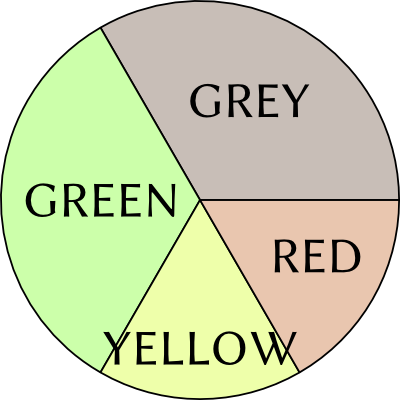
\includegraphics[width=100px]{./spinner.png}
 % spinner.png: 400x400 pixel, 81dpi, 12.55x12.55 cm, bb=0 0 356 356
 \end{center}

 \begin{enumerate}[\hspace{.5cm}a.]
  \item To the nearest $\frac{1}{6}$, what's the probability of spinning green?
  Red?
  \item I spin the spinner twice. What's the probability of spinning green, then
  red?
  \item I spin the spinner twice. What's the probability of spinning red, then
  green?
  \item I spin the spinner twice. What's the probability of spinning red and
  green (in any order)?
 \end{enumerate}
\end{problem}

\begin{problem}{Challenge}
 Jennifer records the colours of cars that pass her house between 8:00 AM and
 9:00 AM for one week. Her results are as below:
 \vspace{0.5cm}
 \renewcommand{\arraystretch}{1.2}

 \begin{center}
  \begin{tabular}{|c|c|c|c|c|}
  \hline
  Day of Week & Red Cars & Green Cars & Blue Cars & Total \\ \hline
  Monday & 10 & 2 & 2 & \hspace{4cm} \\
  Tuesday & 8 & 4 & 4 & \\
  Wednesday & 9 & 1 & 0 & \\
  Thursday & 11 & 2 & 0 & \\
  Friday & 10 & 1 & 1 & \\
  Saturday & 2 & 0 & 6 & \\
  Sunday & 2 & 0 & 5 & \\ \hline
  Total & & & & \\ \hline
  \end{tabular}
 \end{center}

 \begin{enumerate}
  \item Fill in all missing total values.
  \item Assume that these patterns hold every week. Find the probability that a
  car passing on Tuesday will be red. To do this, divide the red cars that
  passed on Tuesday by the total number of cars passing on Tuesday.
 \end{enumerate}

 This type of problem is called conditional probability.

\end{problem}

\end{document}
